\section{Zielsetzung}
In diesem Experiment soll die Erzeugung freier Elektronen durch Erwärmung von Metalloberflächen untersucht werden.
Dabei werden vorallem Kennlinien einer Hochvakuumdiode und die Austrittsarbeit betrachtet.

\section{Theoretische Grundlagen}
\subsection{Austrittsarbeit}

\noindent
Da im Kristallgitter des Metalls ein einheitlich positives Potential herrscht, 
wirken auf die Elektronen keine Kräfte und sie können sich dort frei bewegen.
Das Potential des Ausßenraums ist von dem des Metallinneren verschieden, 
wodurch ein Elektron beim verlassen des Metallbandes gegen das Potential $\xi$ anlaufen und Austrittsarbeit leisten muss.
In Abbildung (\ref{fig:pottopf}) ist der Potentialverlauf mithilfe eines Potentialtopf-Modells dargestellt.

\begin{figure}
    \centering
       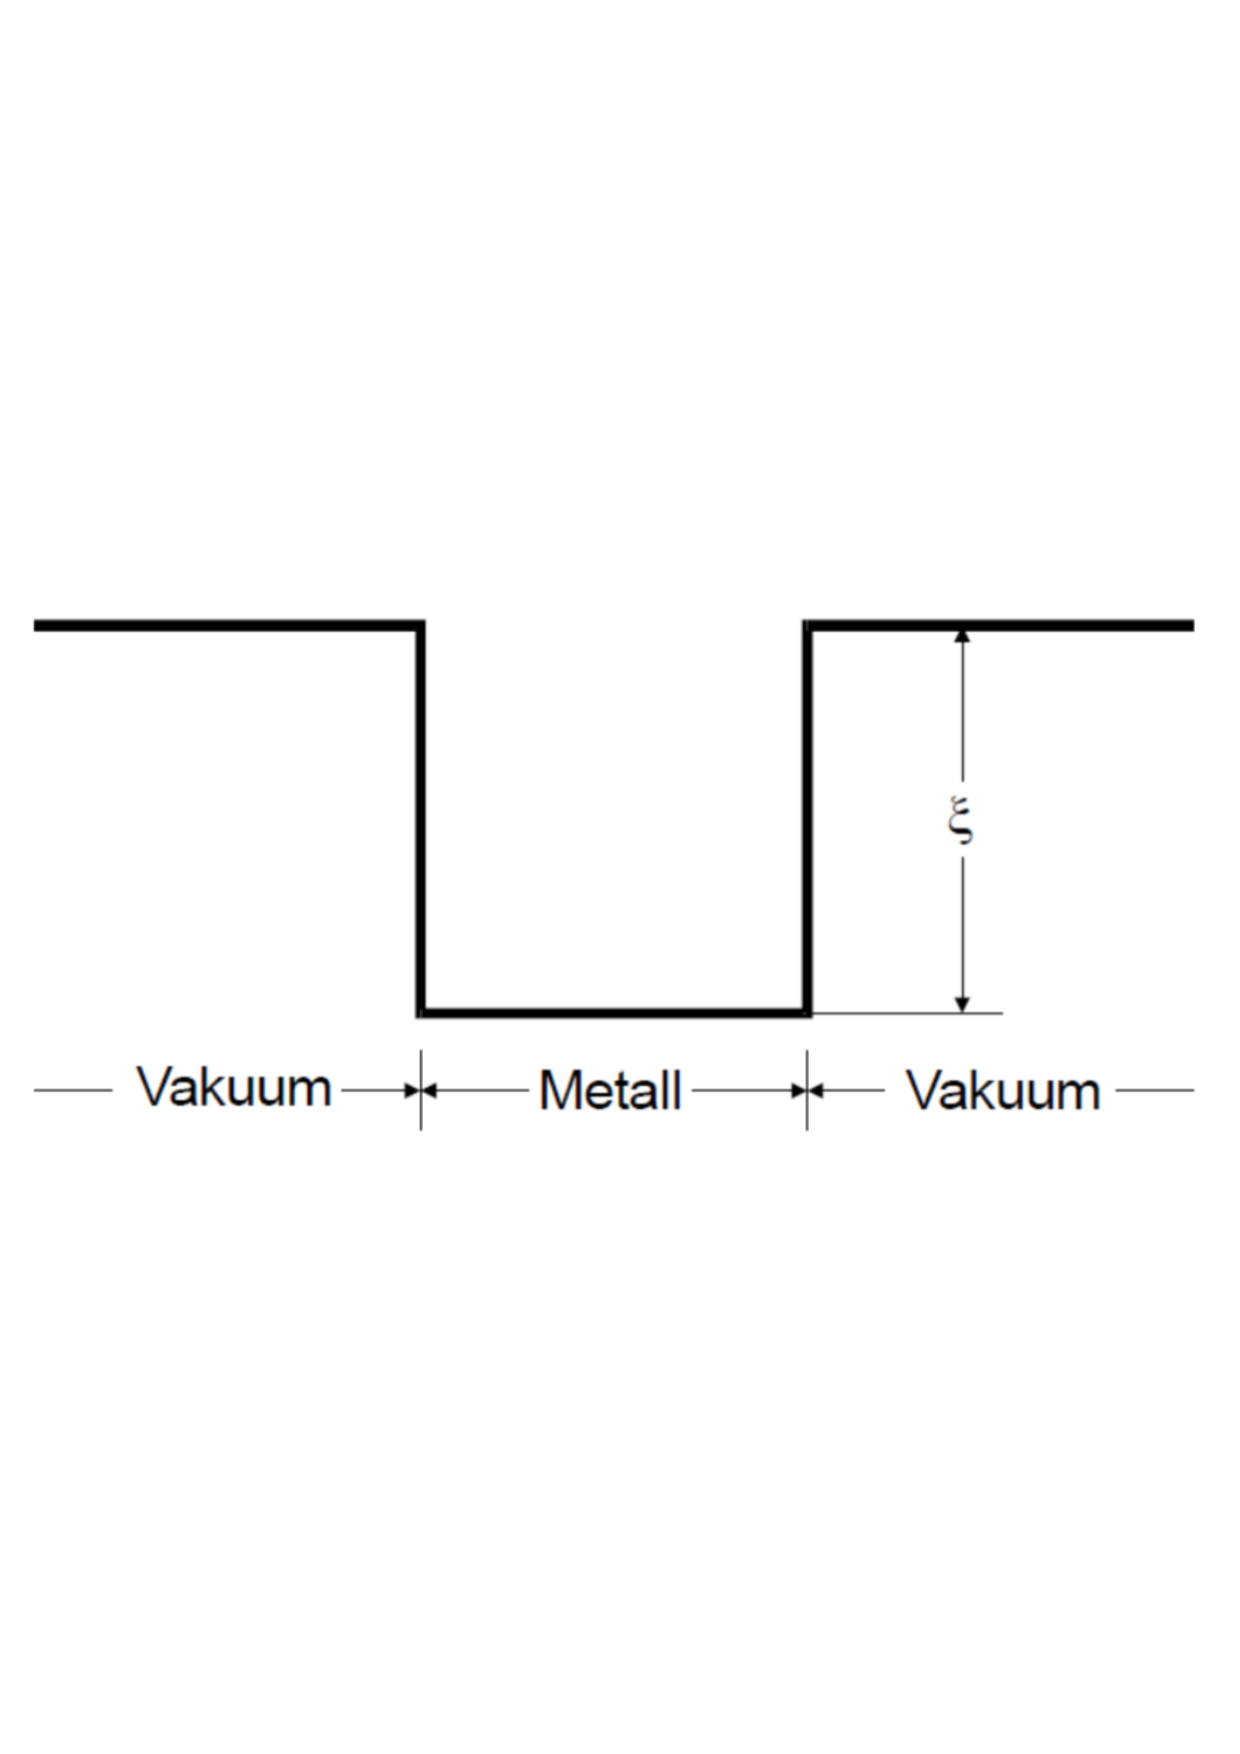
\includegraphics[height=5cm]{pottopf.pdf}
       \caption{Potentialtopf-Modell (Quelle: \cite{V504}).}
       \label{fig:pottopf}
\end{figure}

\noindent
Die Wahrscheinlichkeit dafür, dass ein Elektron ein mögliches Energieniveau besitzt, 
ist nach der Quantentheorie durch die Fermi-Diracsche Verteilungs-Funktion 

\begin{equation}
\text{f}(\text{E})=\frac{1}{\text{exp}(\frac{\text{E}-\zeta}{\text{kT}}) + 1}
\label{eqn:fermi}
\end{equation}

\noindent
gegeben.
Da die Fermische Grenzenergie $\zeta$, 
die Maximalenergie der Elektronen bei T=0 in Abhängigkeit von der Zahl n der Elektronen pro Volumeneinheit im Metall, 
für alle Metalle bei Zimmertemperatur $\zeta >> \text{kT}$ ist 
und beim Schmelzpunkt des Wolframs noch so groß gegenüber kT ist, 
kann die Näherung

\begin{equation}
\text{f}(\text{E}) \approx \text{exp} \biggl( \frac{\zeta-\text{E}}{\text{kT}} \biggr)
\label{eqn:fermi2}
\end{equation}

\noindent
angenommen werden.
%
\subsection{Die Hochvakuumdiode}

\noindent
Da freie Elektonen mit Luftmolekülen wechselwirken, kann der glühelektrische Effekt nur im Vakuum untersucht werden.
Dazu befindet sich ein Draht (hier Wolfram)    in einem evakuierten Glaskörper, der durch einen Strom erwärmt werden kann.
Die aus der Glühkathode austretenden Elektonen werden durch eine von außen anliegende Saugspannung zur Anode beschleunigt, 
wo dann ein Strom gemessen werden kann. 
Der Aufbau einer solchen Hochvakuumdiode ist in Abbildung (\ref{fig:diode}) dargestellt.

\begin{figure}
    \centering
       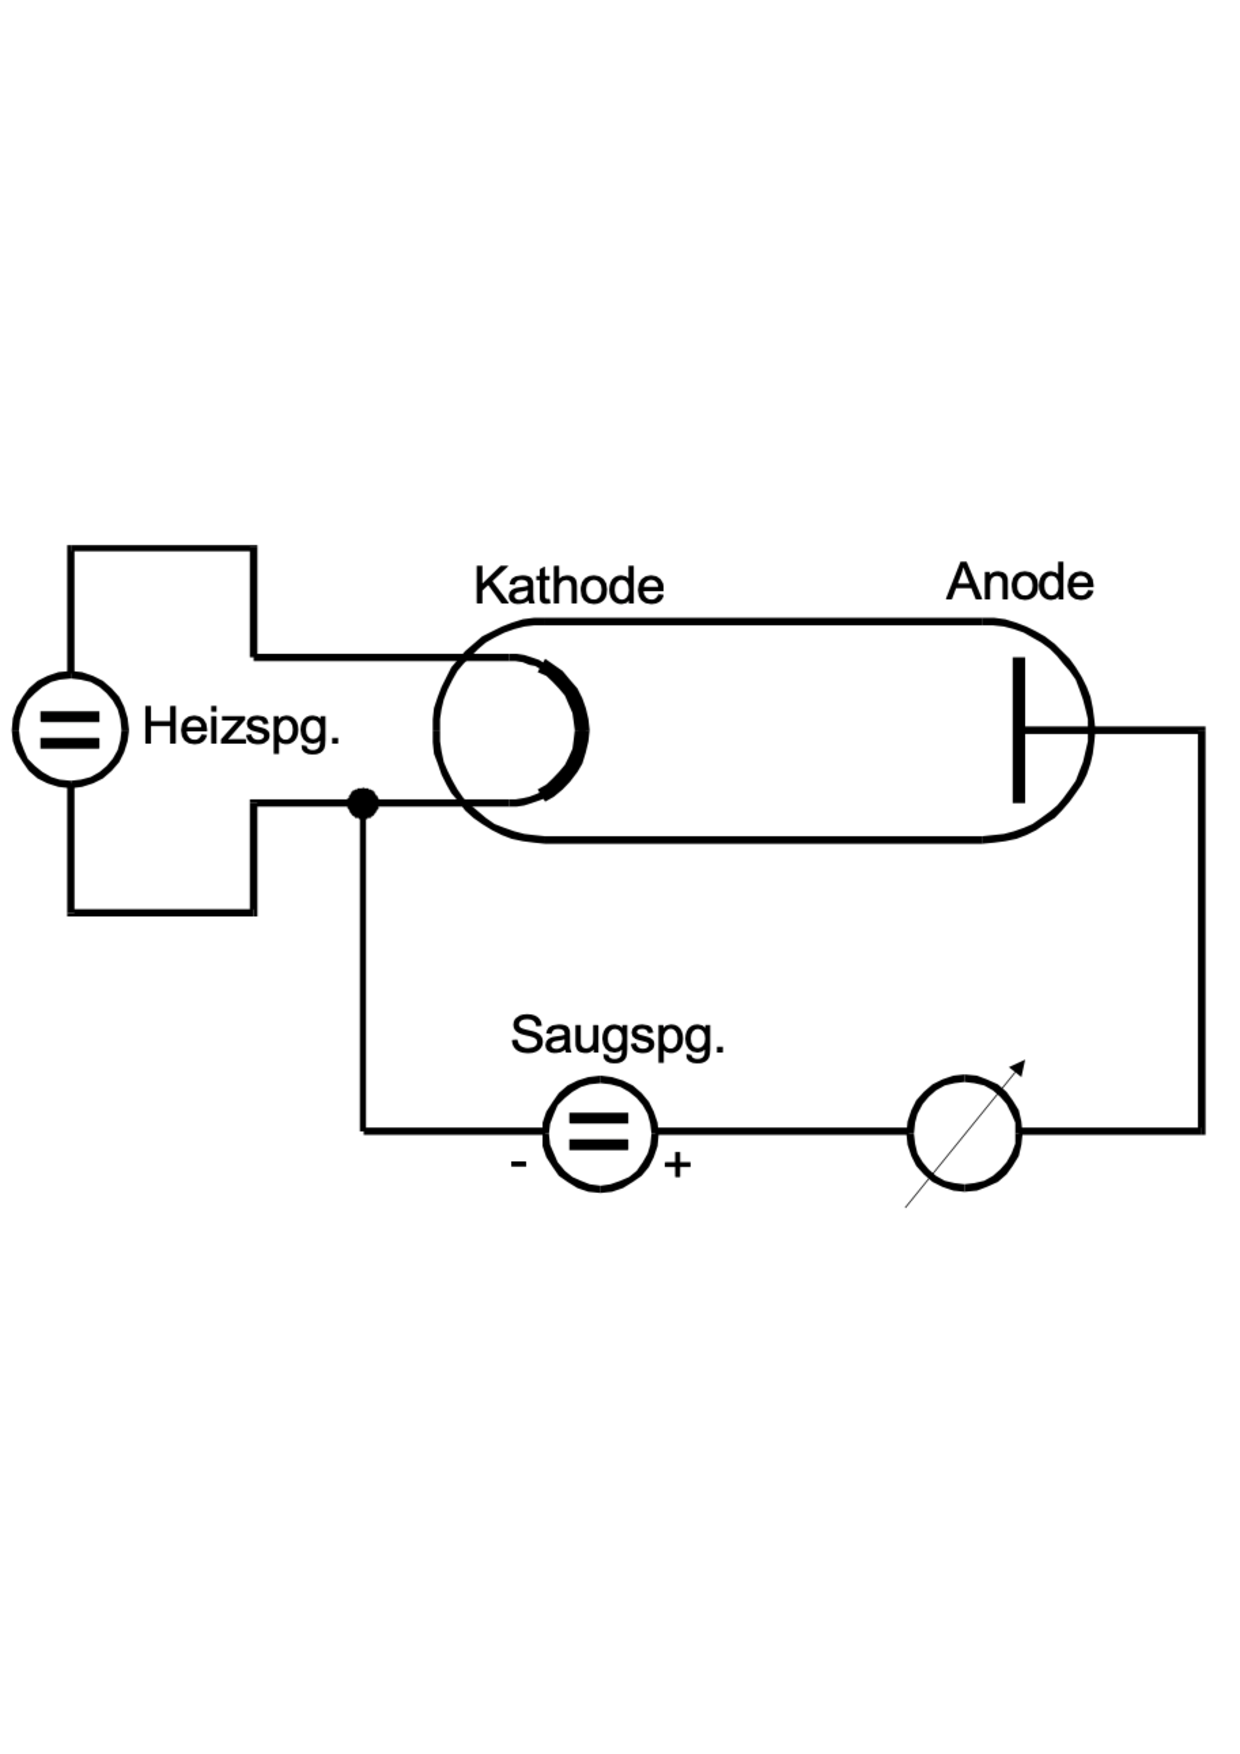
\includegraphics[height=5cm]{diode.pdf}
       \caption{Aufbau einer Hochvakuumdiode (Quelle: \cite{V504}).}
       \label{fig:diode}
\end{figure}

\noindent
Der Zusammenhang zwischen dem Anodenstrom $\text{I}_\text{A}$ und der Saugspannung U wird als Kennlinie bezeichnet.
Ihr Verlauf wird in Abbildung (\ref{fig:kenn}) dargestellt.

\begin{figure}
    \centering
       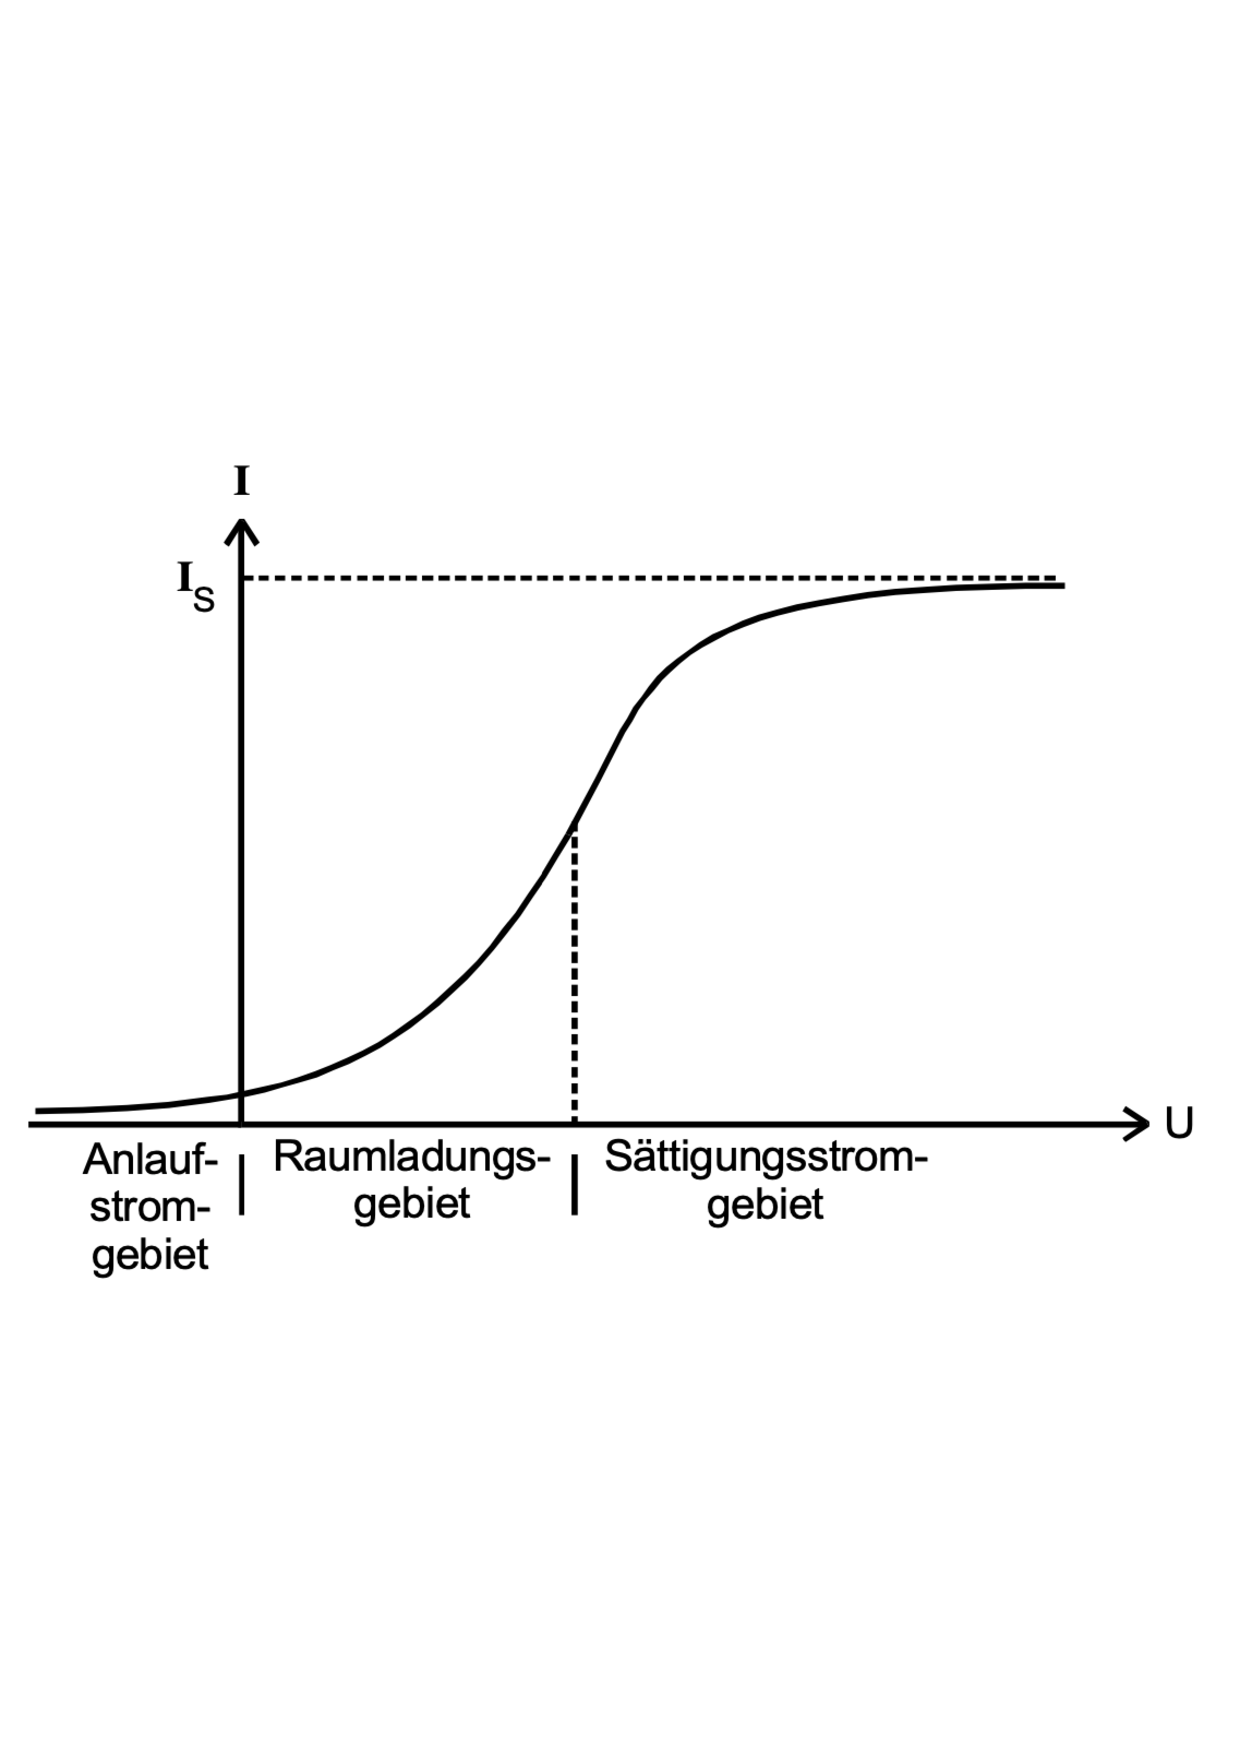
\includegraphics[height=5cm]{kenn.pdf}
       \caption{Kennlinie einer Hochvakuumdiode (Quelle: \cite{V504}).}
       \label{fig:kenn}
\end{figure}

\noindent
Es ist fällt auf, dass sich die Kennlinie in die drei Bereiche Anlaufstrom- Raumladungs- und Sättigungsstromgebiet unterteilen lässt,
welche in den folgenden Kapiteln näher untersucht werden.


\subsection{Die Sättigungsstromdichte}

\noindent
Die Zahl der Elektronen, die in Abhängigkeit von der Temperatur T pro Zeit- und Flächeneinheit aus einer Metalloberfläche austreten, 
wird als Sättigungsstromdichte $\text{j}_\text{S}(\text{T})$ bezeichnet.
Diese lässt sich aus der Bedingung (\ref{eqn:bed}) herleiten, die besagt, dass nur Elektronen aus der Metalloberfläche austreten können, 
die eine so große Geschwindigkeitskomponente in Z-Richtung haben, sodass

\begin{equation}
\frac{\text{p}_\text{z}^2}{2\text{m}_0} > \zeta + \text{e}_0 \phi
\label{eqn:bed}
\end{equation}

\noindent
gilt. Darüber wird so integriert, dass die Sättigungsstromdichte schließlich die Richardson-Gleichung ergibt.

\begin{equation}
\text{j}_\text{S}(\text{T}) = 4\pi \frac{\text{e}_0 \text{m}_0 \text{k}^2}{\text{h}^3} \text{T}^2 \text{exp} \biggl( \frac{-\text{e}_0 \phi}{\text{kT}} \biggr)
\label{eqn:rg}
\end{equation}

\subsection{Die Langmuir-Schottkysche Raumladungsgleichung}
Die Raumladungsdichte $\rho$ der Elektronen nimmt zur Anode hin ab, 
sodass sie den Verlauf der Feldstärke beeinflusst und das Feld von der Kathode abschirmt.
Da die emittierten Elektronen dann nicht mehr alle vom Anodenfeld erfasst werden,
ist der gemessene Diodenstrom kleiner als der nach der Richardson-Gleichung (\ref{eqn:rg}) berechnete Sättigungsstrom.
Die Poissonsche Gleichung

\begin{equation}
\Delta \text{V} = - \frac{1}{\varepsilon_0} \rho
\end{equation}

\noindent
gibt den Zusammenhang zwischen Anodenspannung und -strom an.
Daraus ergibt sich anstelle des Ohmschen Gesetzes, was hier bei beschleunigten Elektronen nicht gültig ist,
das Langmuir-Schottkysche Raumladungsgesetz

\begin{equation}
\text{j}= \frac{4}{9} \varepsilon_0 \sqrt{\frac{2 \text{e}_0}{\text{m}_0}} \frac{\text{V}^{\frac{3}{2}}}{\text{a}^2}
\label{eqn:lsr}
\end{equation}

\noindent
wobei $ \text{j} \sim \text{V}^{\frac{3}{2}}$ und das Gesetz im Raumladungsgebiet gilt.

\subsection{Das Anlaufstromgebiet}

\noindent
Obwohl nach dem Langmuir-Schottkysche Raumladungsgesetz (\ref{eqn:lsr}) für U = 0 auch j = 0 ist, 
fließt in Realität noch ein geringer Anodenstrom, 
welcher durch die Eigengeschwindigkeit der Elektronen beim verlassen der Kathode entsteht.
Diese Elektronen erreichen selbst bei einem kleinen Gegenfeld die Anode und der dabei gemessene Anodenstrom wird Anlaufstrom genannt.
In Abbildung (\ref{fig:anlauf}) ist der Potentialverlauf im Anlaufstromgebiet dargestellt.

\begin{figure}
    \centering
       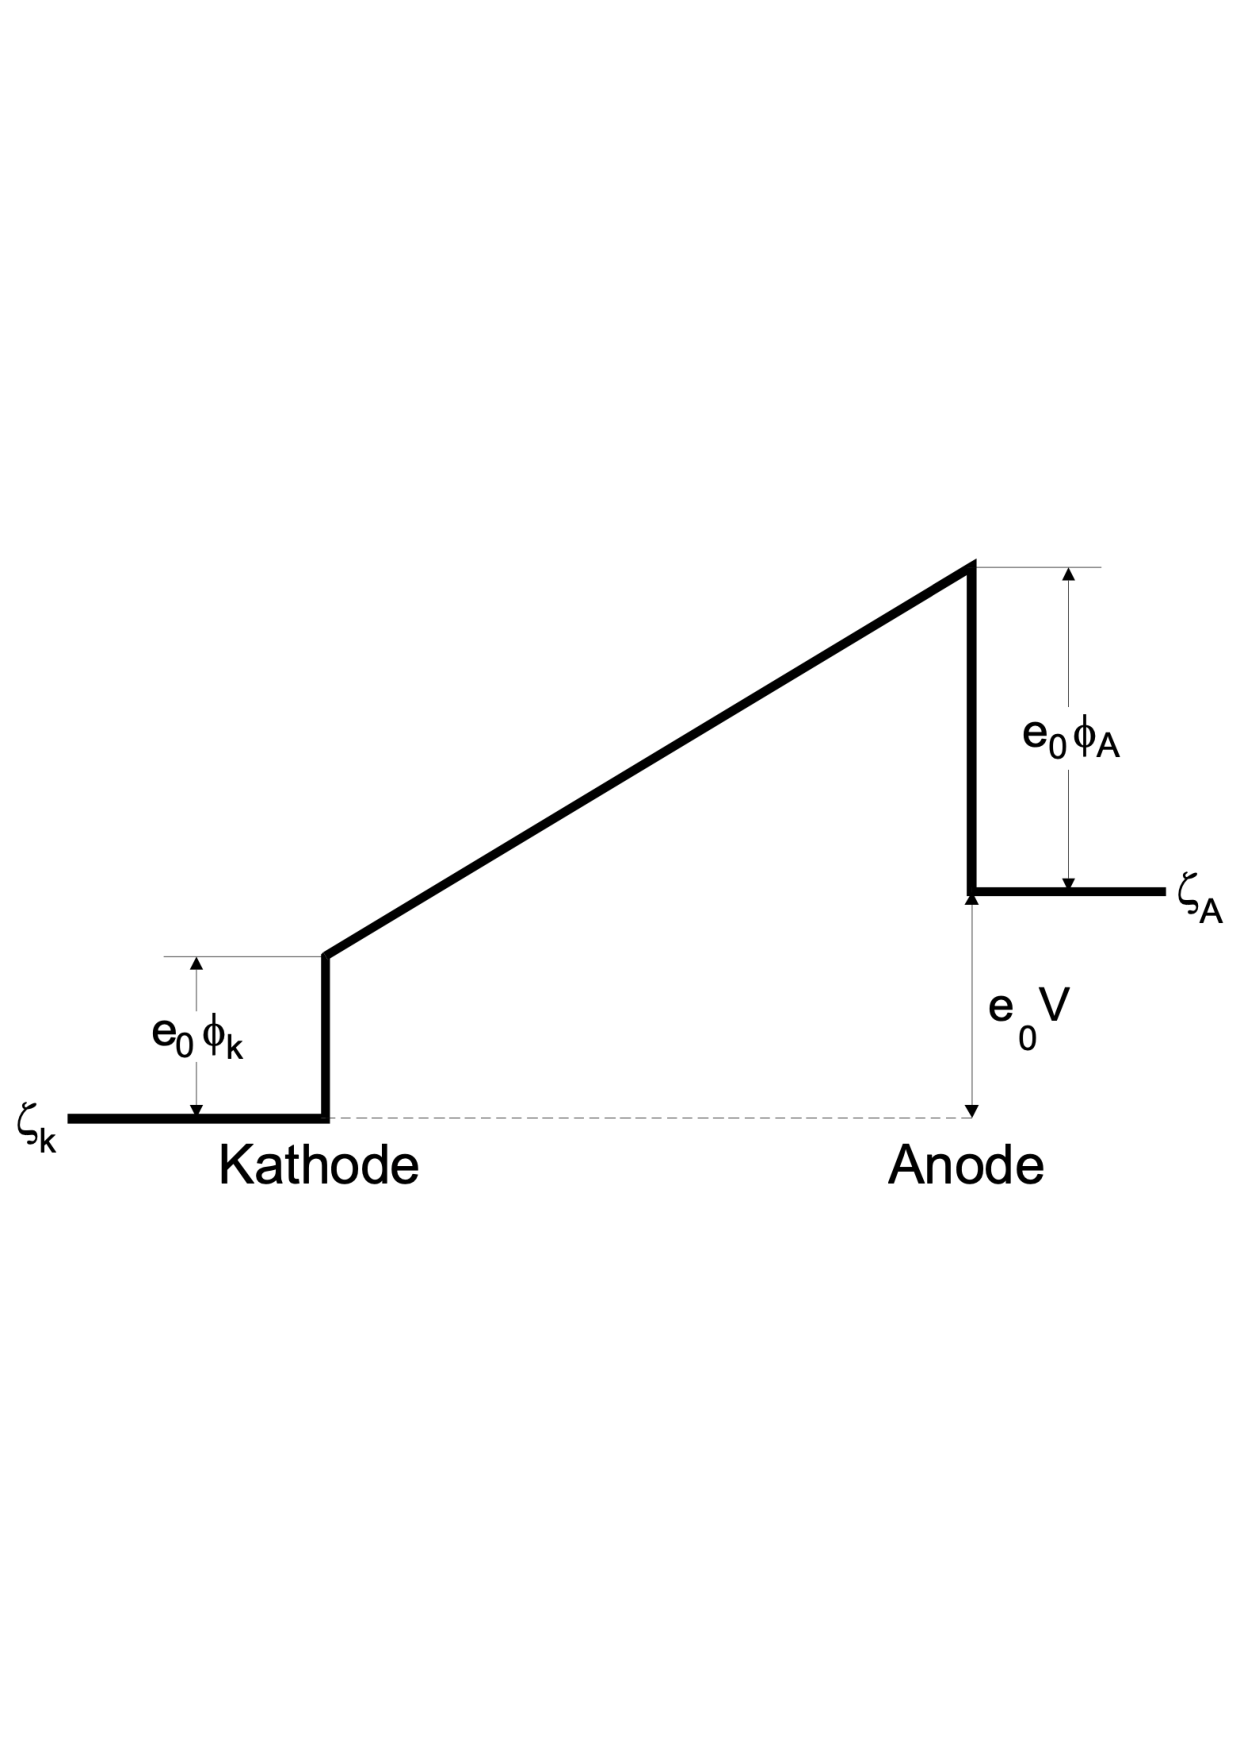
\includegraphics[height=5cm]{anlauf.pdf}
       \caption{Potentialverlauf im Anlaufstromgebiet (Quelle: \cite{V504}).}
       \label{fig:anlauf}
\end{figure}

\noindent
Die Elektronen müssen also beim verlassen der Kathode mindestens eine Energie von $\text{e}_0 \phi_\text{A} + \text{e}_0 \text{V}$ besitzen,
um die Anode zu erreichen.
Folgende Abhängigkeit der Anlaufstromstärke vom äußeren Potential V ist mit Hilfe Gleichung (\ref{eqn:fermi2}) zu entnehmen.

\begin{equation}
\text{j}(\text{V}) = \text{j}_0 \, \text{exp} \biggl(-\frac{\text{e}_0 \phi_\text{A} + \text{e}_0 \text{V} }{\text{kT}} \biggr) = \text{const.} \, \text{exp} \biggl(-\frac{\text{e}_0 \text{V} }{\text{kT}} \biggr)
\label{eqn:anlauf}
\end{equation}


